
%(BEGIN_QUESTION)
% Copyright 2006, Tony R. Kuphaldt, released under the Creative Commons Attribution License (v 1.0)
% This means you may do almost anything with this work of mine, so long as you give me proper credit

Sketch the traces for controller output and process variable for two scenarios: one where the process is {\it integrating}, and the other where there is {\it dead time} in the process measurement.  In both cases, assume the controller has been placed in manual mode, and given a small step change.  Your sketches should show this step change along with the process variable response:

\vskip 10pt

\noindent
{\bf Integrating process:}

$$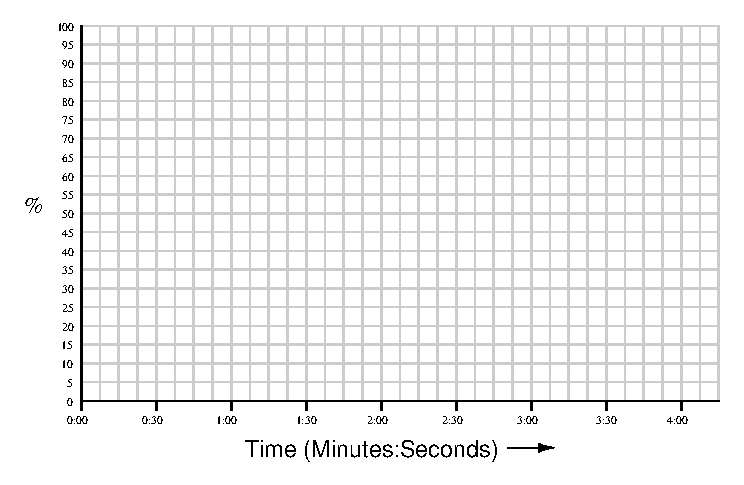
\includegraphics[width=15.5cm]{i00073x01.eps}$$

\vskip 10pt

\noindent
{\bf Process with dead time:}

$$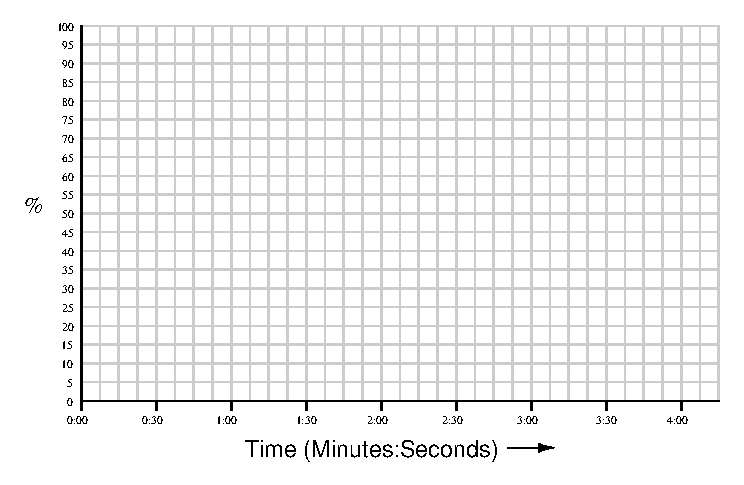
\includegraphics[width=15.5cm]{i00073x01.eps}$$

\vfil

\underbar{file i00073}
\eject
%(END_QUESTION)





%(BEGIN_ANSWER)

This is a graded question -- no answers or hints given!

%(END_ANSWER)





%(BEGIN_NOTES)


%INDEX% Control, PID tuning: process characterization

%(END_NOTES)


